Ben Trout

2014-11-7

Building Intake, Designing 

\begin{tabular}{|p{5cm}|p{5cm}|}
\hline
Building Intake&
As this week got under way we soon realized we wanted to put the intake farther forward and lower to the ground. We lowered the bar farther to the ground and put it to the last hole to the front. It was an easy solution to move the bar lower to the ground as we just added some gears and slipped the intake onto two bars that go into the two side bars. By doing this we gave ourselves a good couple of inches of extra room for the rest of our mechanisms in our robot. 
\\
\hline
Designing&
As we analyzed our robot and realized what limited space we had we soon came to the conclusion as a team that we needed to change shooter mechanisms. We decided that a slingshot was too risky and would not be adequate. We switched to a ramp that the balls would go up and into the tube. As these balls went up the ramp a whacker would spin around and fling the balls up the ramp into the tube. This is still a beginning idea, but has promise. %TODO: WTF Ben? ``Waker''... "is this supposed to be 'wanker' or 'waffer'?" --Hross
\\
\hline
\end{tabular}

\section*{Building Intake}
Our first intake went very well. There was just one problem with it: the intake took up too much space in our robot and we wanted to greatly reduce this. So what we did first is move the intake to the farthest bar forward; that was an easy change. Our second idea to reduce space was to move the intake farther to the ground so we can cut the cardboard and reduce the amount of space it takes up when it revolves around. To move it farther to the ground we added two gears, one attached to the motor and the other attached to the bar the intake was on. We attached two bars to the sides of our robots and attached the intake to those two bars. The two bars on their own would wobble around and I tried to stabilize the bars, but Alex pointed out that once we attached the intake to the two bars it would make the whole mechanism rigid.  Our original intake used a structural bar and we were afraid that it would not allow enough clearance for a big ball to go under. We tried to attach a small bar across the two beams and use that as our main piece for the intake, but it wasn’t strong enough. We ended up just going with our original intake and it does give enough space for the big ball to go under. Our intake is officially done. We cut down the cardboard and there's no way we can move it forward or lower anymore. We are pleased with the intake and will move onto the shooter mechanism next week. 

\section*{Designing}
Our main problems with the slingshot is it took up too much space, didn’t have a reliable way to reload that didn’t take up a ton of space, and didn’t have an easy way to get the balls into the holder that was reliable. As we were messing around with our new intake we soon realized that with the motor on very little power and a lot of weight on it could fling a ball pretty far up a ramp. We rolled with this idea and are now going to build a funnel from the intake to a one ball wide curved ramp in the middle of our robot. A bar over the ramp that has a whacker attached to it will spin around and hit the balls up the ramp. This idea in theory will be much more reliable and efficient. We don’t have to worry about reloading; we can have a constant stream of balls; funneling the balls into the ramp will be easy; and we don’t have to worry about surgical tubing that can wear over time. My only concern with this new design is that balls could easily get clogged in the tube if the whacker can’t hit them high enough or has one misfire and this could lead to a whole lot of trouble. I drew up a design for this and we’ll be starting on it next week. 

\begin{center}
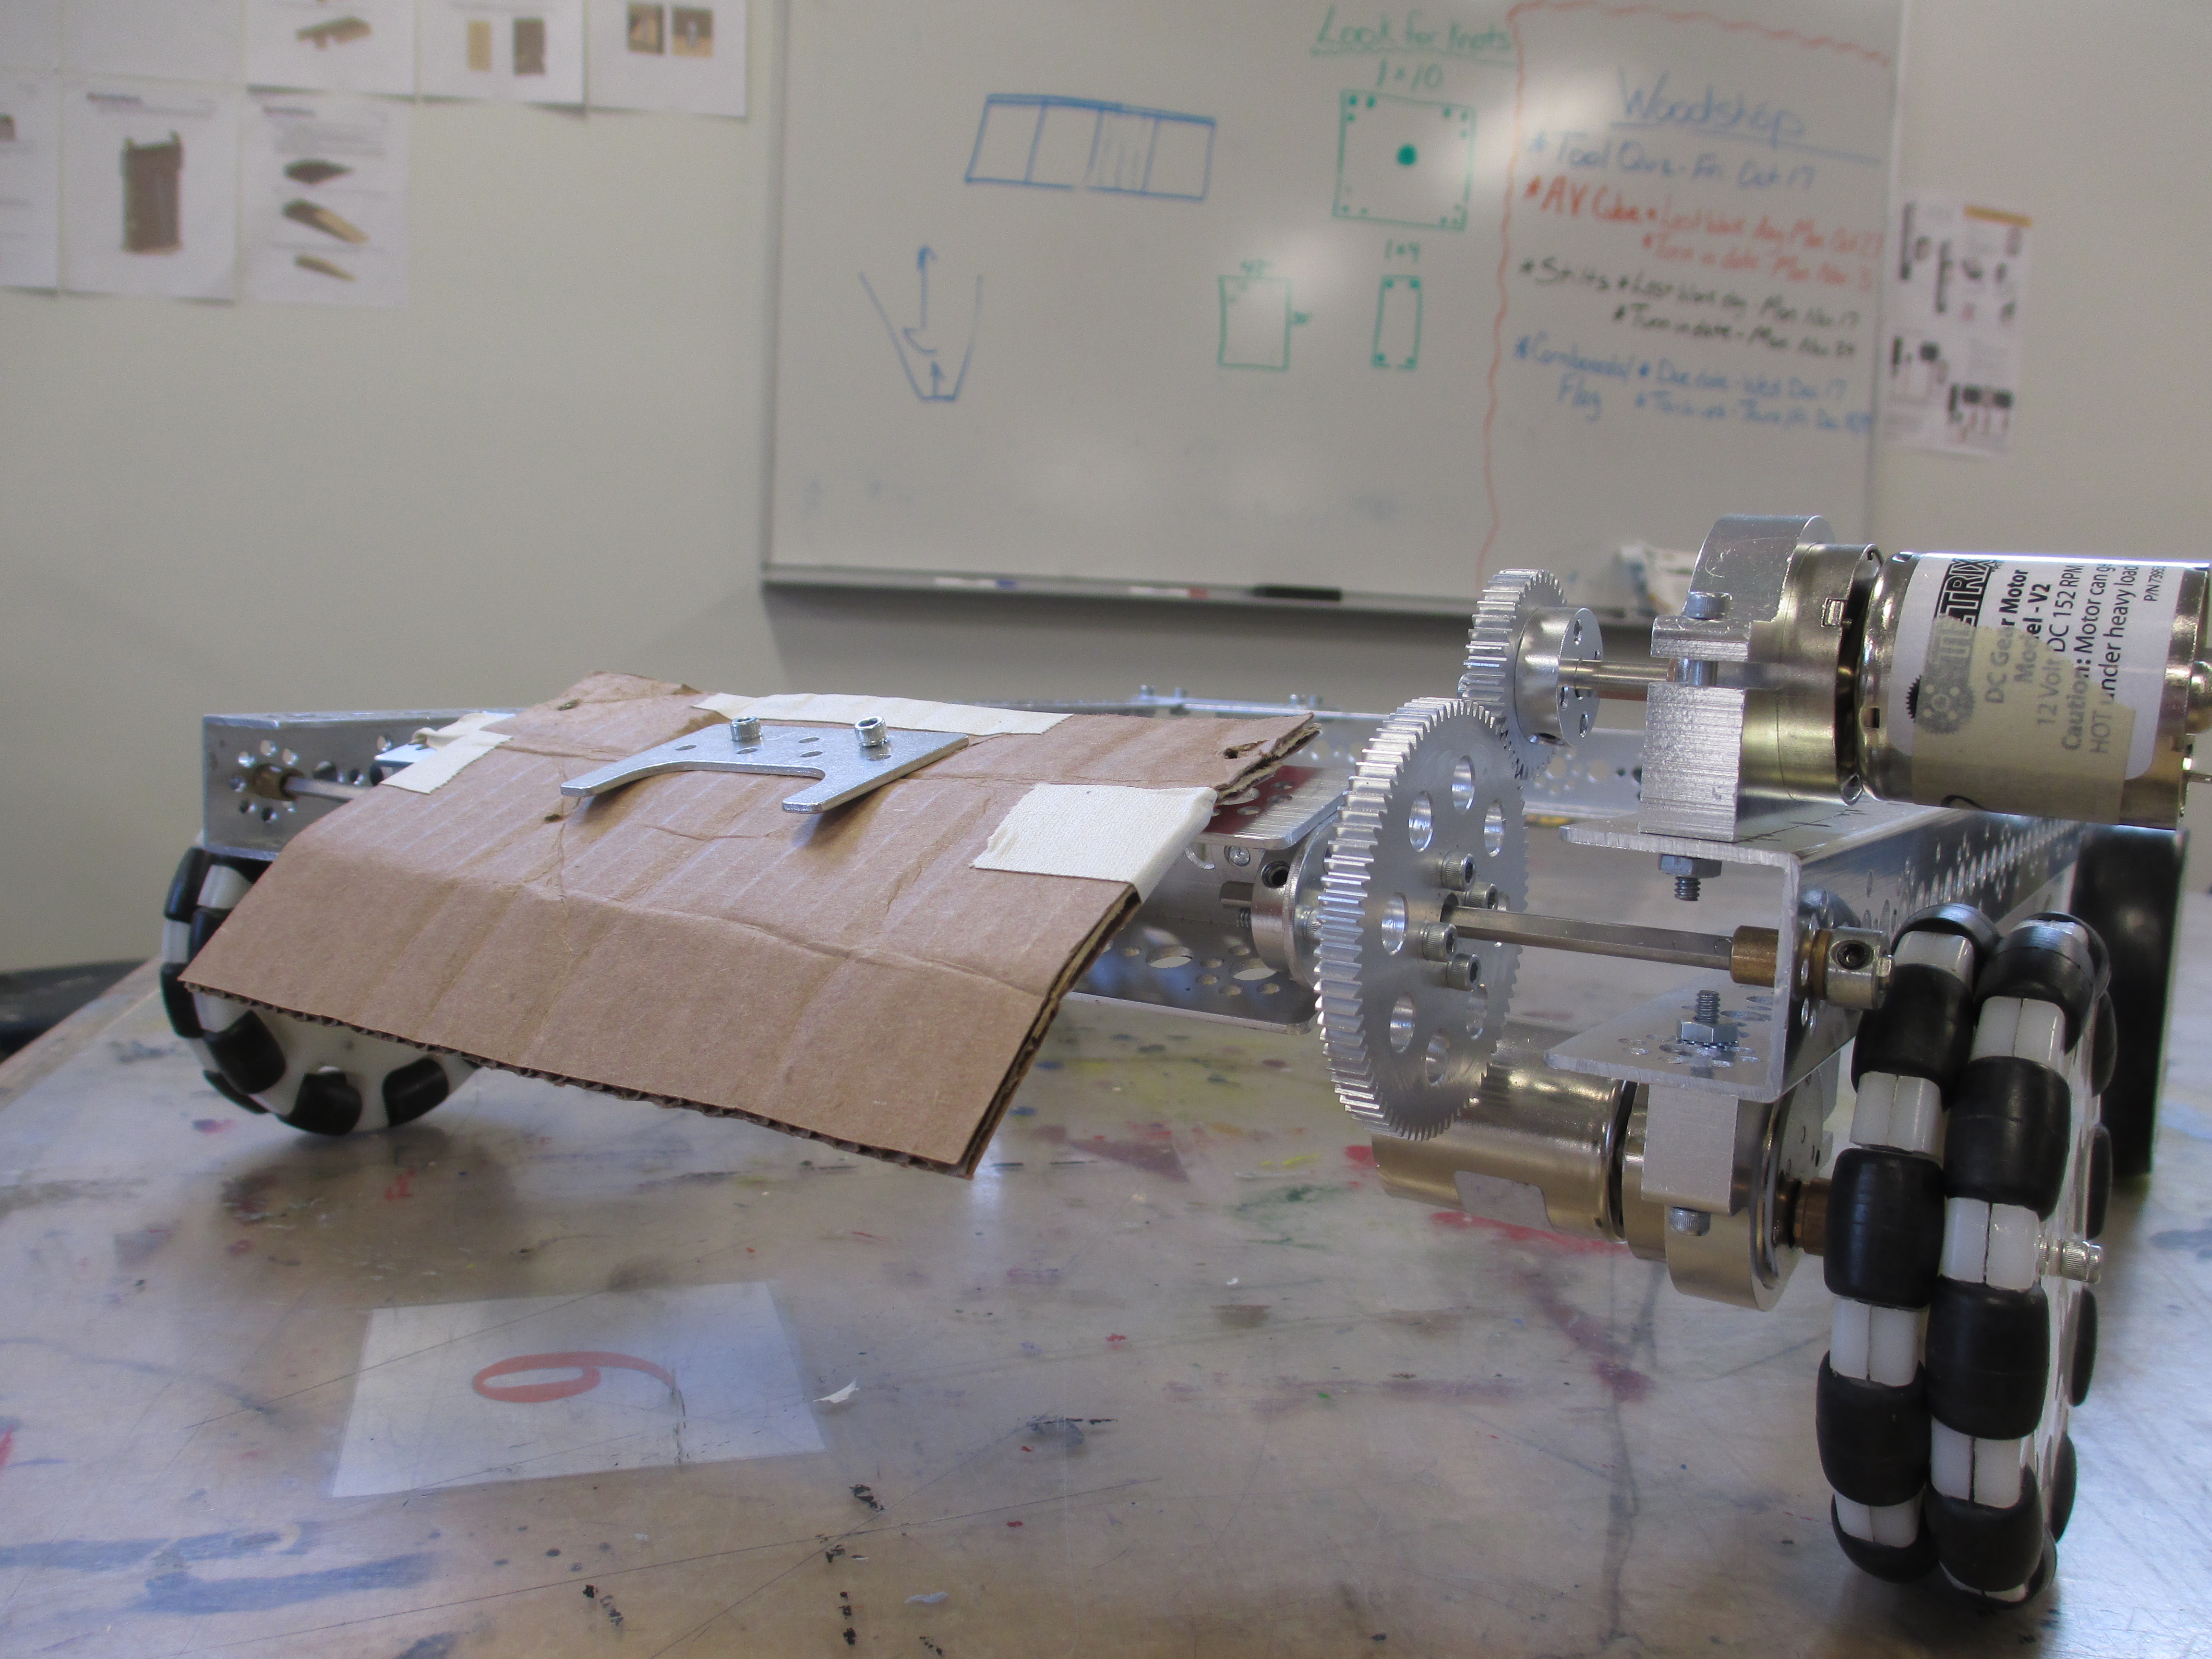
\includegraphics[width=10cm]{./Entries/Images/NewIntake.jpg}
\end{center}
